% Adjust these for the path of the theme and its graphics, relative to this file
%\usepackage{beamerthemeFalmouthGamesAcademy}
\usepackage{../../beamerthemeFalmouthGamesAcademy}
\usepackage{multimedia}
\graphicspath{ {../../} }

% Default language for code listings
\lstset{language=C++,
        morekeywords={each,in,nullptr}
}

% For strikethrough effect
\usepackage[normalem]{ulem}
\usepackage{wasysym}

\usepackage{pdfpages}

% http://www.texample.net/tikz/examples/state-machine/
\usetikzlibrary{arrows,automata}

\newcommand{\modulecode}{COMP260}\newcommand{\moduletitle}{Distributed Systems}\newcommand{\sessionnumber}{5}

\setbeamertemplate{navigation symbols}{}

\begin{document}
\title{\sessionnumber: An Introduction to Digital Sound}
\subtitle{\modulecode: \moduletitle}

\frame{\titlepage} 

\begin{frame}
	\frametitle{Learning outcomes}
	\begin{itemize}
		\item \textbf{Recognise} how audio is used in games
		\item \textbf{Explain} what sound is and how it can be represented digitally
		\item \textbf{Write} a program that will produce a sound
	\end{itemize}
\end{frame}

\part{How are sounds used in Games?}
\frame{\partpage}

\begin{frame}{Audio in Games}

\begin{center}
	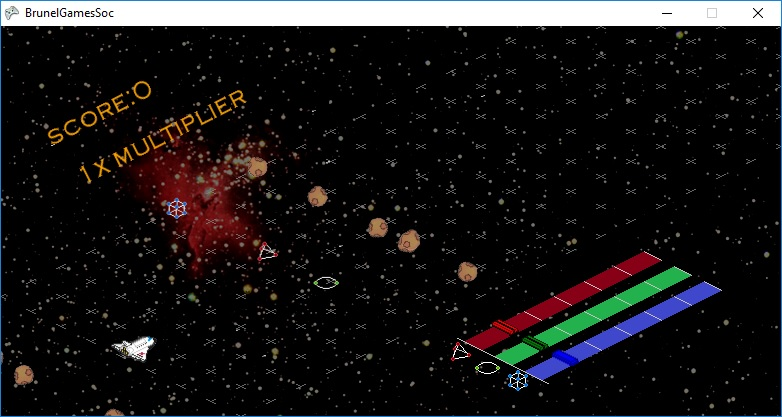
\includegraphics[width=\linewidth,height=0.8\textheight,keepaspectratio]{astroclysm}

	\vspace{1em}

	Astroclysm - X48 2008
\end{center}

\end{frame}

\begin{frame}{Audio in Games}

\begin{center}
	\url{https://www.youtube.com/watch?v=oF7POPv1GyQ}

	\vspace{1em}
		
	\url{https://www.dropbox.com/sh/vrodjzp0zerimik/AAA_OScznYHq9HWgoP0p0K2wa?dl=1}	
\end{center}

\end{frame}

\begin{frame}{Audio in Games}

\begin{itemize}
	\item For the next 10 mins, in pairs:
	\begin{itemize}
		\item Discuss one or two games that use sounds in an interesting way
		\item What was interesting about the use?
	\end{itemize}
\end{itemize}

\end{frame}
\part{What is sound? What is a wave?}
\frame{\partpage}

\begin{frame}
	\begin{center}
		\textbf{Quick Definition:} A wave of compression and refraction in an elastic medium, such as air, which can be detected by an animal’s sense of hearing 
	\end{center}
\end{frame}

\begin{frame}{What is Sound?}
	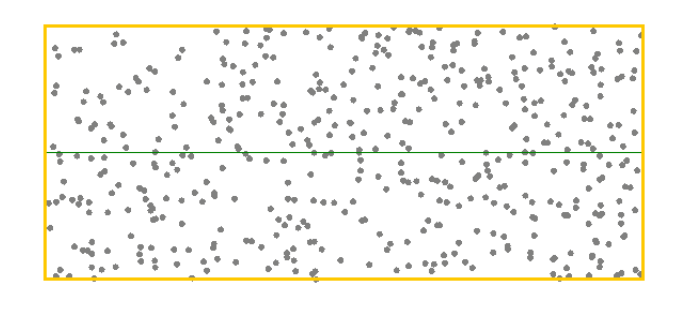
\includegraphics[width=\linewidth,height=0.8\textheight,keepaspectratio]{sound_molecules}
\end{frame}

\begin{frame}{What is a Wave?}
	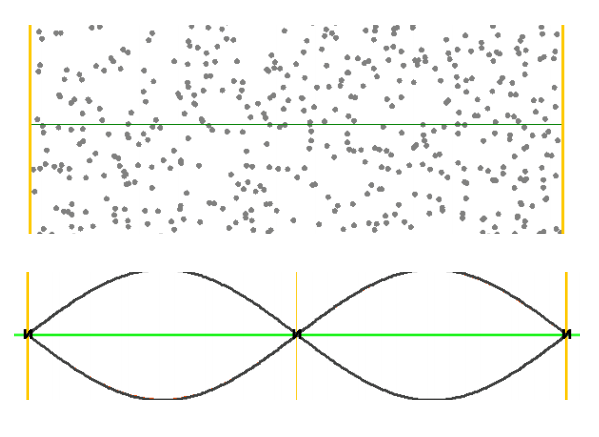
\includegraphics[width=\linewidth,height=0.8\textheight,keepaspectratio]{sound_wave}
\end{frame}

\begin{frame}{What is a Wave?}
	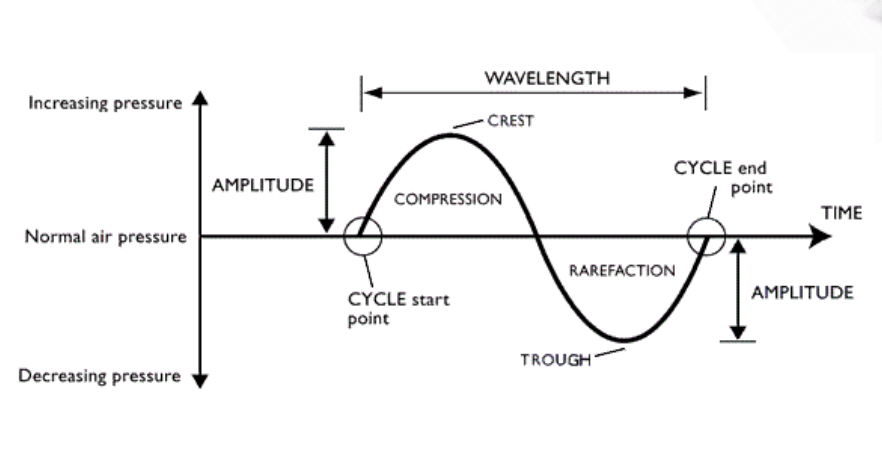
\includegraphics[width=\linewidth,height=0.8\textheight,keepaspectratio]{wave_desc}
\end{frame}

\begin{frame}{What is Sound?}
	\begin{itemize}
		\item Many animals are able to sense sound in two key ways:
		\textbf{volume} and \textbf{pitch}.
		\item\textbf{Volume:} The intensity of the change in pressure, as signified by the
		amplitude of a wave
		\item\textbf{Pitch:} The frequency of the change, as signified by the length of
		the wave and its velocity (i.e., “the speed of sound”)
	\end{itemize}
\end{frame}
\part{How can sounds be represent digitally?}
\frame{\partpage}

\begin{frame}{How Can Sound Be Represented Digitally?}
	\begin{itemize}
		\item One method is to represent the wave itself and one
		approach to do this is \textbf{L}inear \textbf{P}ulse Code \textbf{M}odulation (LPCM).
		\begin{itemize}
			\item An array of integers is created
			\item The value of these integers represents the amplitude of the wave
			\begin{itemize}
				\item  With linear coding, the way how bytes correspond to real-world
				measures - called \textit{quantisation} - is uniform across the range

			\end{itemize}
			\item The positions in the array represent time, and so each element
			contains a sample of the wave amplitude 
		\end{itemize}
	\end{itemize}
\end{frame}

\begin{frame}{How Can Sound Be Represented Digitally? }
	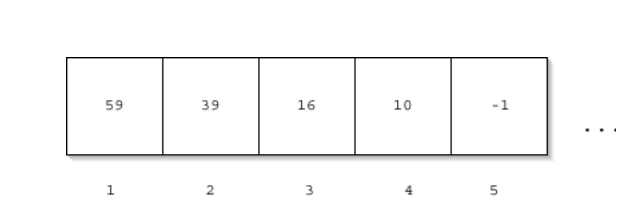
\includegraphics[width=\linewidth,height=0.7\textheight,keepaspectratio]{pcm_array}
\end{frame}

\begin{frame}{How Can Sound Be Represented Digitally?}
	\begin{itemize}
		\item\textbf{Sample Rate:} How many samples are taken per second (consequently,
		how much time is represented by each element in the
		array)?

		\item\textbf{Bit Depth:} How many bits are available to represent the value?
	\end{itemize}
\end{frame}

\begin{frame}{How Can Sound Be Represented Digitally?}
	\begin{itemize}
		\item\textbf{Sample Rate:} i.e., range of frequencies which can be recorded
		array)?

		\item\textbf{Bit Depth:} i.e., the number of amplitude levels which can be
		represented 
	\end{itemize}
\end{frame}

\begin{frame}{How Can Sound Be Represented Digitally? }
	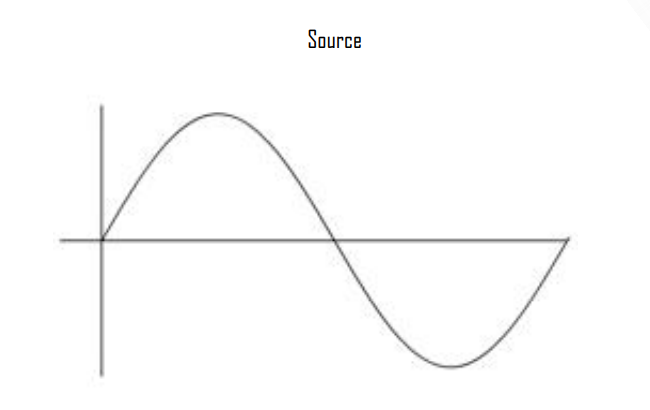
\includegraphics[width=\linewidth,height=0.7\textheight,keepaspectratio]{source_wave}
\end{frame}

\begin{frame}{How Can Sound Be Represented Digitally? }
	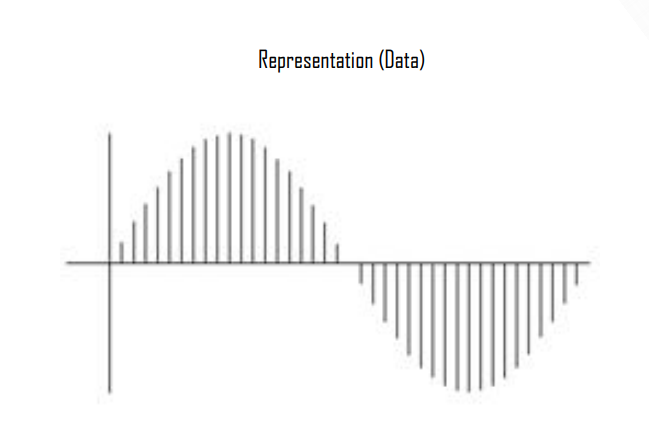
\includegraphics[width=\linewidth,height=0.7\textheight,keepaspectratio]{wave_data}
\end{frame}

\begin{frame}{How Can Sound Be Represented Digitally? }
	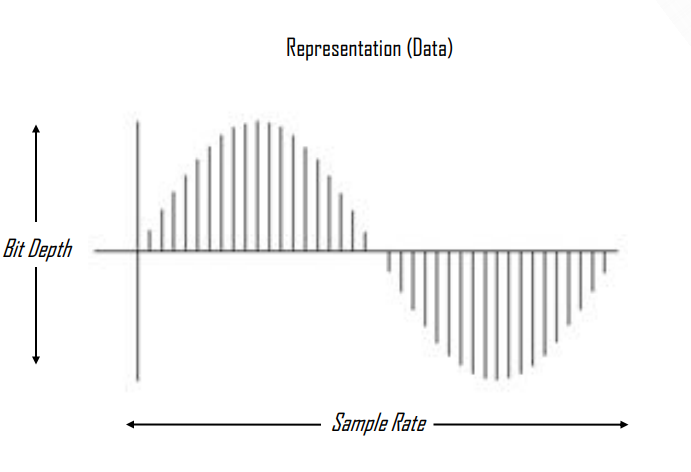
\includegraphics[width=\linewidth,height=0.7\textheight,keepaspectratio]{wave_axis}
\end{frame}

\begin{frame}{How Can Sound Be Represented Digitally? }
	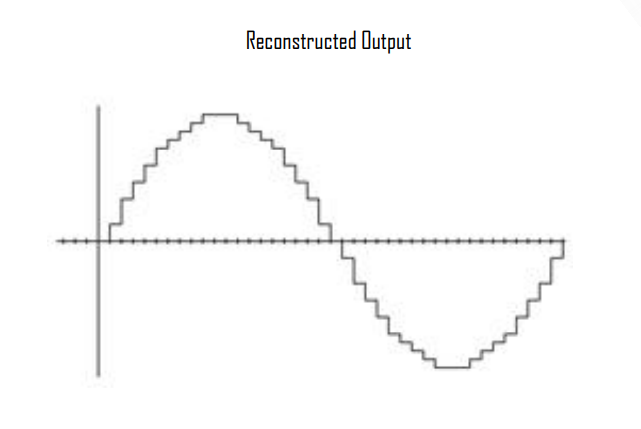
\includegraphics[width=\linewidth,height=0.7\textheight,keepaspectratio]{wave_reconstructed}
\end{frame}
\part{Can I write a program to create sound}
\frame{\partpage}

\begin{frame}
	\begin{center}
		\textbf{Live Coding} - Pygame Mixer
	\end{center}
\end{frame}

\begin{frame}{Exercise 1 - Playing sound and Music}
	\begin{enumerate}
		\item Initialise Pygame and create a basic application which displays a window
		\item Initialise Pygame mixer
		\item Load some music
		\item Play music when a key has been pressed
		\item Load in a sound
		\item Play sound when a key has been pressed
		\item Experiment with some of the mixer and sound functions - \url{https://www.pygame.org/docs/ref/mixer.html}
	\end{enumerate}
\end{frame}

\begin{frame}
	\begin{center}
		\textbf{Live Coding} - SndArray
	\end{center}
\end{frame}

\begin{frame}
	\begin{center}
		\textbf{Live Coding} - Save File
	\end{center}
\end{frame}

\begin{frame}{Exercise 2 - Manipulating Sound}
	\begin{enumerate}
		\item Write an \textbf{algorithm} to increase the volume of the sound
		\item Write this sound to a new file 
	\end{enumerate}
	\textbf{Stretch Goal:} Generate a tone using the sin() maths function and save this sound to a file
\end{frame}
\part{Additional Resources}
\frame{\partpage}

\begin{frame}{Additional Resources}
	\begin{itemize}
		\item\textbf{How sound works: }\url{http://www.explainthatstuff.com/sound.html}
		\item\textbf{Frequently Asked Questions: }\url{http://www.sciforums.com/threads/speakers-how-do-they-produce-different-sounds-simultaneously.97540/}
	\end{itemize}
\end{frame}
\part{PASS Challenge}
\frame{\partpage}

\begin{frame}
	\frametitle{PASS Challenge}
	
	Review the WAVE and PyGame mixer modules at:
	
	\url{https://docs.python.org/3.6/library/wave.html}
	
	\vspace{1em}
	
	\url{https://www.pygame.org/docs/ref/mixer.html}
\end{frame}	
	
\begin{frame}	
	\frametitle{PASS Challenge}
	\begin{itemize}
		\item In pairs
		\item \textbf{Implement} audio i/o in Python
		\item \textbf{Read} a wave file as a wave\_read object
		\item \textbf{Play} audio in PyGame using the PyGame Mixer
		\item \textbf{Write} a new wave file as a wave\_write object
	\end{itemize}
	
	You can learn more about audio:
	
	\vspace{1em}
	
	 \url{https://inventwithpython.com/chapter19.html}
	
\end{frame}

\end{document}
